\section{Project Description \pagebudget{.5}}

Testing plays a central role in modern software development,
contributing crucially both to the costs of software projects and to
the quality of their results.
%
Testing comes in many styles---unit testing, integration testing,
performance testing, stress testing, accessibility testing,
etc.---supported by many sorts of tools, with yet more advanced tools
and techniques continually being developed, discussed, and applied.

One such technique, {\em property-based testing} (PBT), has become
quite popular in the functional programming community since its
introduction in the QuickCheck library~\cite{ClaessenHughes00} in
Haskell and is beginning to make significant inroads in the broader
software industry---for example, the developers of the Hypothesis PBT
tool in Python estimat it has on the order of half a million
users\cite{ZacPersonalCommunication}\todo{Am I remembering that
  right?}.

PBT combines formal software specification\bcp{blah} with random\bcp{?}
testing to achieve low-effort, high-impact bug-finding.
\bcp{Rich theoretical foundation, etc. etc.}
%
It has been used, for example, to find critical bugs in telecommunications
software~\cite{arts2006testing}, replicated
file-stores~\cite{hughes2014mysteries}, cars~\cite{arts2015testing}, and a range
of other programs~\cite{hughes2016experiences}.
%
Select companies make PBT part of
their testing workflow and find it to be an invaluable tool for ensuring
correctness~\cite{Bornholt2021}.

\todo{
  \begin{itemize}
    \item Increasing the impact of PBT in industry would improve productivity
    and make software more robust. What would that take?
    \item We're in the middle of an in-depth formative study to find out just
    that
    \begin{itemize}
      \item Still doing analysis, but some broad themes have become clear
      \item List high-level theme categories
    \end{itemize}
    \item The goal of the project is to capitalize on that data and advance PBT
    by:
    \begin{enumerate}
      \item Understanding the foundation: challenges PBT faces in industry
      \item Addressing difficulties in specification, generation, and testing
      validation with theoretically motivated and rigorously designed tools
      \item Setting up comprehensive resources for education
    \end{enumerate}
    \item In the following section, we describe the study in some detail and use
    it to motivate the work that we propose in this project
    \item MOTIVATION SECTION
    \begin{itemize}
      \item Motivating questions for JS study
      \item Lay out study parameters in some (but not much) detail
      \item Discuss some emerging themes
      \begin{itemize}
        \item Give justification in the form of quotes for some
        \item Say why the themes are important, how they line up with existing
        understanding
        \item Situate themes relative to their categories
      \end{itemize}
      \item Tie everything together
      \begin{itemize}
        \item The themes of this study map onto the projects that we plan to
        carry out
        \item Each theme category has a section below, each project in those
        sections directly serves one or more of the themes in that category
        \item Here's what we're going to do...
      \end{itemize}
    \end{itemize}
  \end{itemize}
}

\subsectionstar{Orientation: What is Property-Based Testing? \pagebudget{.4}}\label{sec:orientation}

\bcp{I think we need a longer overview of PBT, here, for readers that
  are not familiar.}

\subsectionstar{Motivation: A Formative Study of PBT in Industry \pagebudget{2}}\label{sec:motivation}

\hg{Pulled from the section below, we'll need to massage}
The first step is to conduct qualitative interviews to understand the challenges
that programmers face when using PBT tools. To this end, we plan to undertake an
interview study with our research partner, Jane Street, LLC\footnote{See letter
of support in the appendix.} to develop a deep understanding of the challenges
programmers face using PBT in industrial settings as well as being to explore
potential solutions.

\textbf{Research questions}.
Our key research question will be, \emph{How can the research community make PBT
more valuable for software developers?} More specifically, we seek
answers to the following questions:

\begin{itemize}[noitemsep,leftmargin=4em]
\item[\bf RQ1.] What support do developers need to help them imagine properties? \todo{Reword, the notion of ``imagining'' properties has not yet been introduced.}
\item[\bf RQ2.] What kinds of generators do testers need to exercise their
  properties effectively? Do they have specific precondition and/or distributional
  requirements?
\item[\bf RQ3.] What aspects of the developer workflow around PBT need improvement?
\item[\bf RQ4.] What concrete changes could be made to modern PBT systems
  to improve effectiveness and usability?
\end{itemize}

{\bf RQ1}, {\bf RQ2}, and {\bf RQ3} relate to property,
generator, and workflow challenges, respectively.
{\bf RQ4} more directly asks how existing systems might
be improved. This final question will help to keep us focused,
reminding us that participants likely have the context and knowledge not
only to identify challenges but also to suggest
solutions.

\textbf{Research site}. We will partner with Jane Street, LLC, a large
financial technology firm.
Jane Street has a number of qualities that makes it an ideal place for
this study. To start, Jane Street developers use
a variety of testing tools, including PBT. This gives us a place to start
when asking questions, since participants will likely have seen PBT before,
and it means that will be score for exploring trade-offs between PBT and
other forms of testing.
Additionally, Jane Street developers famously build almost all of their
systems in OCaml, a mostly functional programming language with strong support
for static typing and modularity. This unified ecosystem
will allow
us to control for a number of potentially confounding factors: all of the
developers we talk to will have access to the same PBT tools and the same
libraries, language-level programming abstractions, house coding rules,
etc. (which might make testing easier or harder).

Naturally, carrying out a study at a single firm has potential drawbacks as
well. The most obvious is that our results may not generalize: We
cannot guarantee that our findings will apply outside of the OCaml ecosystem (and
other ecosystems like it). However, Jane Street is home to a diverse array of
software systems, including trading systems, quantitative
algorithms, networked systems, and hardware description code~\cite{signalsandthreads}.
We hope that the breadth of these programming tasks will mean that the software
developers that we talk to will come to the discussion with a wide variety of
experiences.


\subsubsectionstar{Context: Property-Based Testing}%
%
Property-based testing (PBT) is a form of random testing~\cite{hamlet1994random}
that was popularized by the QuickCheck~\cite{DBLP:conf/icfp/ClaessenH00} library
in Haskell. In PBT, users write executable functions that act as partial
specifications of a function under test. For example, a tester might write the
following property to specify the \lstinline{insert} function for an
implementation of a binary search tree (BST):
\begin{lstlisting}
  prop_insertCorrect x t = isBST t ==> isBST (insert x t)
\end{lstlisting}
This property is an ordinary function that takes an integer and a tree as input
and asserts that if the original tree satisfies the BST invariant, then so does
the tree after inserting the integer. There are a myriad of different kinds of
properties that one might use to specify a system; a good source of examples is
\citet{HowToSpecifyIt}.

With a property in hand, a tester then passes a series of inputs to the property
and checks that the property evaluates to \lstinline{True} for each input.  If
some input causes the property to fail, then it constitutes a {\em
counterexample} to the property and potentially a bug in the program. If no
counterexample is found after the tester's time budget has elapsed, the tester
will have gained confidence that the property holds in general.

In this dissertation I focus on the case of random PBT, where the series of
inputs that check the property are generated by some random process, but there
are alternatives. In particular, {\em enumerative testing} advocates
deterministically listing every possible input from the smallest to the largest,
relying on the ``small scope hypothesis''~\cite{jackson1996elements} that most
bugs can be found with ``small'' inputs. There are a variety of systems that use
this technique~\cite{DBLP:conf/haskell/RuncimanNL08,leancheck}. Forms of model
checking can also be considered alternatives to random PBT; their approaches
vary but at their core model checkers are often tools for searching an input
space for counterexamples~\cite{biere2009bounded}.

Despite the success of the enumerative testing and model checking, random
generation is still a dominant player in the PBT space. Its success is often
attributed to the fractal nature of ``big'' test cases---many structures are
self-similar, so testing with one big structure also tests the code with the
exponentially many smaller sub-structures. This effect is powerful, but it still
takes a bit of work to get random generation ``right.'' Many have pointed out
that the distribution that inputs from drawn from is incredibly important for
effective testing, so programmers are often forced to choose a distribution
manually~\cite{DBLP:conf/icfp/ClaessenH00}. Even more importantly, testers need
to ensure that the sampled inputs are {\em valid} to test with; I discuss this
problem in the next section.

\bcp{Related work to mention: HypoFuzz \url{https://hypofuzz.com}}

\subsectionstar{Contributions}

%
\todo{Outline project goals with pointers to relevant
  sections. Include a pointer to the work plan section below.}

\subsectionstar{Personnel}

\todo{A short paragraph about what a great team we are, how the PI
  qualifications complement each other, and what kind of students we aim to
  support.  }

\subsection{Foundation: Understanding Needs and Opportunities \pagebudget{1}}

As PBT sees wider adoption, new opportunities present for understanding how
these tools are being used in practice, and how these tools can be further
developed to better support developers' needs. In this section, we describe a
sequence of studies we will undertake to better understand developers' needs.
These studies will draw on mixed methods in the service of producing a
comprehensive and actionable agenda for future research.  Phases of this
research include interviews to develop an initial taxonomy of needs and
obstacles to tool use (Section~\ref{sec:interviews}), a survey to assess the
generality of these needs and obstacles and to identify potential for adoption
of PBT tools (Section~\ref{sec:survey}), and observations to understand
particular tasks involved in PBT to an extent that we can understand how to
design new algorithms and interactive tools that better support those tasks
(Section~\ref{sec:observations}).

\subsubsection{Ongoing Work: Need-Finding Interviews with Jane Street}
\label{sec:interviews}

We will begin our need-finding work by interviewing developers who can shed
light into how PBT is already being used, and obstacles in its use. Interview
studies are common in early-stage need-finding research, due to their ability
to yield highly informative stories about people, the tasks they need to
accomplish, and the tools they use to accomplish them. The purpose of these
interviews is to identify a broad set of opportunities for improving PBT tools,
grounded in concrete, authentic, detailed stories from developers.

\textbf{Method}. Semistructured interviews will be conducted with approximately
30 developers. Questions will focus on tasks these developers wish to accomplish
with PBT tools, and around developers' recollections of what it was like to
work with PBT tools to accomplish these tasks.

\textbf{Population}. Ideally, these interviews would involve both current users
of PBT as well as non-users of PBT. In reality, it is difficult to recruit and
have meaningful conversations with non-users of a technology. We plan to
recruit users across as broad a spectrum of usage as we can reasonably recruit,
including both frequent users of PBT technologies, as well as a handful of
developers who have had only limited, occasional exposure to PBT. Our survey
study (Section~\ref{sec:survey}) aims to establish contact with a broader
sample of non-users of PBT to assess opportunities for making PBT tools more
valuable and discoverable for this group.

\textbf{Progress}. Our interview instrument and analysis process was developed
and tested with 7 users of the Hypothesis PBT toolkit, recruited over Twitter.
This analysis yielded a conceptual framework of barriers to usage of PBT, which
we published recently at HATRA, an ACM SPLASH workshop and one of the key
venues for presenting preliminary research on human aspects of formal methods
tools and type systems~\cite{goldstein2022some}.

We have since established a collaboration with Jane Street, LLC\footnote{See
the attached letter of support.} with whom we will conduct an expanded
interview study. To date, through this collaboration we have already conducted
27 of 30 interviews, including both developers who have had exposure to PBT as
well as developers of PBT tools. Our interview process has included an on-site
visit where we collected feedback on our evolving conceptual framework of the
needs and opportunities we have discerned around PBT tools.

What remains for this project is another approximately 2 months of Ph.D.
student work, including conducting the remaining interviews, performing
in-depth qualitative analysis of the data following a thematic analysis
approach~\cite[Chapter 5]{blandford2016qualitative}, and preparing a manuscript
for submission to OOPSLA.

\textbf{Preliminary results}. Key takeaways emerging from our initial analysis
appear in Section~\ref{sec:motivation}.\amh{Is there anything else we want to
say here about the results?}

\subsubsection{Proposed Work: Survey for generalizing findings}
\label{sec:survey}

% \subsubsection{Proposed Work: Characterizing the Potential for Impact in Improved PBT Tools}

\amh{Mention that we plan to distribute a survey among users of Hypothesis to
assess the extent to which our findings generalize among a broader population of
users of PBT tools. Can we get a letter of support from Zac?}

\amh{I think we need to conduct two studies, one focused on assessing the
extent to which our findings about obstacles generalize across PBT users
broadly, and one assessing the extent of potential adoption of these tools,
if major obstacles to adoption are lowered.}

We will conduct a survey with the purpose of understanding the impact that
improved PBT tools could have in industry, if major usability issues were
addressed. We see this survey as crucial in understanding the amount of
resources that should be devoted to PBT research. Furthermore, this
questionnaire will help shed light into which of the usability challenges from
the interview study, if addressed, are most likely to impact a broad set of
current and prospective users of PBT tools.

\subsubsection{Proposed Work: Observations of PBT in practice}
\label{sec:observations}

\amh{The areas where I think we could most benefit from better understanding
PBT tasks in detail are (1) generator design, implementation, and evaluation;
(2) evaluating the results of properties (in particular, debugging and addressing
counterexamples). I think that our success in designing appropriate tools for
developers might depend on us having a clearer understanding of what it looks
like for developers to undertake these tasks.}

The next step is to more deeply characterize the obstacles faced with specific
tools and tasks through close observation. We anticipate conducting observations
of participants formulating properties and creating generators, as we expect
that close observation of developers performing these tasks will yield yet
additional detail about ways that developers are supported and not supported by
the tools they use today to a level of depth we will not achieve with the
interviews.

\subsection{Specification: Step 1, Widening the On-Ramp to Properties \pagebudget{2}}
\subsubsection{Proposed Work: When to Specify It!}
Since PBT is often described as a kind of lightweight formal method, one might
have imagined that a central challenge of using PBT would be coming up with the
right specifications. Indeed, our preliminary study concluded just that. But at
Jane Street we actually heard very little about the challenge of coming up with
properties; instead, most participants described applying PBT in scenarios when
properties were already available or quite easy to imagine. This suggests that,
while PBT education should certainly spend some time teaching developers how to
write specifications for arbitrary programs, it should spend even more energy
helping developers quickly recognize  situations where PBT is a particularly
natural fit because properties are obvious.

With this in mind, we plan to write a short paper (with an accompanying talk)
entitled {\em When to Specify It!}. The paper will be a spiritual successor to
John Hughes's {\em How to Specify It!}~\cite{HowToSpecifyIt}, a lovely account
of the many different kinds of properties that one can write for a given piece
of code. Clearly it is important to ask {\em How}, but the developer interviews
suggest that it may be even more important to have a clear sense of {\em When}
to use PBT. {\em When to Specify It!} will combine examples from developer
interviews with ones from our our years of experience studying and applying PBT
into the definitive guide for the most impactful opportunities to apply PBT.
% \begin{itemize}
% \item Code that is already (semi-)formally specified.
% \item Functions that round trip.
% \item Pure data structures.
% \item Modules with invariants.
% \item Related versions of the same code.
% \item Programs that may fail catastrophically.
% \item Stateful APIs with well-understood contracts.
% \end{itemize}

\subsubsection{Proposed Work: Properties Over Printed Output}
\subsubsection{Proposed Work: Making Model-Based PBT First-Class}

\hg{Andrew wrote this for a slightly different thing}
Motivation: How do you design a generator DSL in an imperative language? A
generator uses higher-level functions in a way that might be confusing to people
who used Python.  (e.g., passing a generator of numbers to a generator of lists
to get randomized lists of numbers). Is there a way of designing APIs for
generators that can make the composition of these types of generators easier to
reason about and express for some programmers?

(Joe says the DSLs are well-designed, but the code is hard to debug. How do you
write a generator that works really well, that has a good data distribution and
finds bugs? See below.)

Plan of work. Not sure. This might require some discussions with more uses of
Hypothesis-like libraries.

Next steps—get examples of sloppily-expressed PBtests in Python and then think
through how they would be written more clearly.

\subsubsection{Proposed Work: Interactive Property Specification}

\bcp{General comment for this section: It all seems good, but it is a bit vague
and high level---I feel like technical readers will want a bit more meat.  Could
we spice it up with a concrete example?  (Indeed, should we be thinking about a
running example for the whole proposal?)} \amh{Agreed, I think a concrete
example would be \emph{great} here. Maybe there is an example we can bring in
from the QuickSpec paper~\cite{claessen2010quickspec}}

As our preliminary interview study has suggested, developers sometimes have
difficulty imagining which properties to test, even when they know that their
software would benefit from property-based testing. One area we are interested
in exploring is how programmers can work with their PBT tools to decide on a set
of significant properties to test.  Prior research demonstrates that automated
tools can extract specifications of a program's
behavior\cite{ammons2002mining,le2018deep,claessen2010quickspec}. We are
interested in the non-trivial research problem of integrating such techniques
into usable developer tools. We see the research as addressing several
challenges:

\textit{Generated properties should be \emph{important}}. Any non-trivial
program can be characterized by an overwhelmingly large number of properties,
many of which describe only incidental aspects of the program's behavior that do
not need to be tested. How can tools produce those properties that developers
would want to have tested? We believe that this is a problem that can be best
solved with a mixed-initiative approach~\cite{allen1999mixed}, where properties
are determined by judiciously incorporating both developer input and automated
techniques.

Developer could guide a specification mining tool to extracting relevant
properties through input mechanisms such as (1) identifying regions of code that
are likely to lead to an adverse behavior such as an exception or a logical
error; (2) providing unit test cases that test a special case of a generalized
property; and (3) indicating aspects of interest on input and output data during
exploration in a debugging REPL.

\textit{Generated properties should be \emph{readable}}. While prior research
has shown promise for automatically generating specifications of program
behavior, we expect that users of PBT systems would benefit from having
properties generated in the language of their property-based testing tools.
Furthermore, there are some variants about systems that may be so complex that
they require significant comprehension time for users (i.e., those involving a
large number of clauses). In such cases, a tool may way to generate simpler
variants of properties first, and allow developers to refine them on their own.

\textit{Tools should help developers \emph{revise} properties}. If a generated
property is too relaxed, the tool should request that developer provides a
counterexample that should trigger a failure, and then regenerate the property.
If a generated property is too strict, a tool should allow a programmer to mark
a counterexample that was generated by the PBT tool as spurious, i.e., not
indicating an actual failure of the program. In each of these cases, the
property generator may have generate multiple properties for a developer to
review, each of which may satisfy the refinements that a developer has provided.

\textit{Plan of work}: We will iteratively design and develop developer tools as
an extension to the VSCode editor, a popular development environment for
Haskell. In our first iterations, candidate properties will be generated using
QuickSpec~\cite{claessen2010quickspec}. The interactions described above will be
designed and tested first for simple programs, and then on successively more
complex programs from our benchmark set. PI Head has extensive experience
designing and developing developer tools involving program
analysis~\cite{head2018interactive,head2019managing} and program
synthesis~\cite{head2017writing} components, and extending the VSCode
environment~\cite{head2020composing}.  \bcp{Maybe consider focusing on OCaml
tools, rather than Haskell, since this is where there might be synergy with Jane
Street?  Or do both?} \amh{This is a great idea. Does anyone know of any
specification generators for OCaml?}

\subsection{Generation: Step 2, Better Tools for Random Inputs \pagebudget{3}}
\hg{Intro here}

\subsubsectionstar{Context: Why is random generation hard?}%
Before presenting our proposed work to improve the state of random data
generators, we must first discuss the major difficulties with random generation
for PBT and the existing work that aims to address those difficulties.
\todo{Link all of this to the intro}

{\em Validity Constraints.}
Many properties that developers want to test have {\em preconditions}
(equivalently {\em validity conditions} or {\em input constraints}) that
restrict the set of inputs that should be used for testing. This comes up often
when testing data structures with invariants that must hold in order to apply
the operations under test.  Testing such properties can be problematic, because
many preconditions are difficult to satisfy randomly; if the developer is not
careful they may waste considerable time and energy generating and throwing away
invalid inputs. We call the challenge of quickly generating lots of
precondition-satisfying inputs the {\em valid generation problem}.

{\em Coverage of Realistic Inputs.}
Even among valid inputs, not all are equally realistic. Often generated inputs
feel fabricated, since they are not constructed with prior knowledge of the
kinds of inputs that the program is likely to see. Ideally, developers should be
able to quickly and easily tune their generators to better mimic the real world.

{\em Other Distributional Concerns.}
And {\em even} with validity and realism accounted for, there are other ways for
generators to under-perform. In particular, the spaces of inputs that generators
target is often very large, and the best generators explore the whole space as
quickly as possible. This often (but not always) leads users to manually tune
the weights on generators' choices to ensure that the generator does not spend
too much time in one part of the space or another.

The literature addresses these concerns to various degrees, and the tools to
fall on a spectrum from automatic to manual. The automatic approaches use
proxies for validity and general ``interestingness'' of inputs: some optimize
readily available metrics like code coverage~\cite{afl-readme}, others ask users
to provide metics~\cite{loscher2017targetedpbt}, and, naturally, a few use
machine learning to infer proxies validity~\cite{godefroid2017learn,
DBLP:conf/icse/ReddyLPS20}. Slightly more manual approaches are based on
declarative representations of validity conditions: for preconditions that are
primarily structural, {\em grammar-based fuzzing} provides a compelling
solution~\cite{godefroid2008grammar, holler2012fuzzing, veggalam2016ifuzzer,
wang2019superion, srivastava2021gramatron}, and for more complex, semantic
preconditions, some have proposed using SMT-solvers
programming~\cite{dewey2017automated, LuckPOPL, steinhofel2022input} to
automatically seek out valid inputs. This semi-automatic category also includes
tools for {\em example-based tuning}, a process that improves realism of inputs
by mimicking user-provided examples~\cite{soremekun2020inputs}.

The most flexible, but the most manual, solutions use hand-written generators,
written in a convenient domain-specific language. These are the topic of the
next section.

\subsubsectionstar{Context: Monadic Generators}
When writing generators manually, it helps to have a clean domain-specific
language (DSL) for writing them down. In the Haskell language, where PBT was
first popularized, many such DSLs are implemented using {\em
monads\/}~\cite{moggi1991notions}, which are an elegant design pattern for
expressing effectful (in this case, random and stateful) computations in a pure
language. While monadic DSLs are not necessary to express generators in non-pure
languages, some libraries (e.g., in OCaml) still use monadic abstractions to
build their generator DSLs.

Monadic generators implement arbitrary random data producers (e.g., it is
possible to write a monadic generator for well-typed System F terms), so they do
not compromise on expressiveness over other representations. Yet, monadic
generators are syntactically constrained in a way that isolates the
probabilistic code and prevents usage errors (like passing the wrong random seed
around). As we will see, the constrained nature of monadic generators makes them
the perfect candidates for sophisticated manipulations and interesting
generalizations.

\subsubsection{Prior Work: Free Generators}
In order to improve monadic generation along the dimensions listed above, we
must first re-frame generators as {\em parsers of randomness}. A generator
operates by making a series of random choices, but we can equivalently think of
it as being provided some random sequence of choices and then simply following
those choices to produce a value. This perspective has been used in a few
implementations of PBT systems~\cn{}, but we made it formal in our paper, {\em
Parsing Randomness}~\cite{goldstein2022parsing}.

The paper introduces {\em free generators}, which generalize the standard
monadic generator abstraction, demonstrate a formal link between parsing and
random generation, and enable new algorithms for generation that address the
valid generation problem. Free generators are written the same way as standard
monadic generators, but they are more like generator ``plans'' or syntax
trees.%
\footnote{Free generators are implemented using {\em freer
monads}~\cite{kiselyov2015freer}, which have been used to great effect in recent
years to capture the structure of effectful computations
(cf.~ITrees~\cite{old:xia2019interaction}). Freer monads represent
monadic
computations syntactically by reifying the monad operations (\lstinline{return}
and \lstinline{>>=}) as data constructors. Critically, this is all implemented
within the language (no macros or AST manipulation). See the paper for more
details on the free generator representation.}
This means that a single free generator can be be {\em interpreted} in multiple
different ways. In {\em Parsing Randomness} we prove that any free generator can
  be interpreted either as a standard monadic generator or as a source of
random choice strings with a parser over those strings; this formalizes the
relationship between generators and parsers. Furthermore, since free generators
are uninterpreted syntax trees, they can be manipulated programmatically. Free
generators admit a version of a Brzozowski
derivative~\cite{brzozowski1964derivatives} that can be used incrementalize
generation. We show that free generator derivatives enable an algorithm called
{\em Choice Gradient Sampling}, which uses repeated derivatives to guide a
generator to inputs that are more likely to be valid with respect to a given
precondition.

\subsubsection{Ongoing Work: Reflective Generators}
Continuing on from the free generator work, we have begun to look at even more
powerful generalizations of the standard monadic approach to random generation.
One such project, which is already well underway, concerns monadic generators
that can be run {\em backward}.

If a generator parses a sequence of choices into a value, then running the
generator backward should take a value and produce a sequence of choices that
would produce that value. With this in mind, we present {\em reflective
generators}, an extension of monadic generators that can be run backward to
``reflect'' on the choices that they made when producing an input. The machinery
that makes reflective generators work is quite complex,%
\footnote{Reflective generators are both monads and {\em partial profunctors},
and implement bidirectional programming in the style of Xia et
al.~\cite{xia2019composing}. This approach to bidirectional programming is
related to lenses~\cite{foster2009bidirectional}, but it hides much of the
complexity of bidirectional program composition in the bind operation of the
monad. The result is an elegant programming experience where both directions of
the computation can be written at once in a type-safe way.} but, like free
generators, their syntax is still quite close to that of normal monadic
generators.

Reflective generators are useful for more than just generation; we currently
have two working examples of useful applications.

\noindent {\em Validity-Preserving Mutation} Many automated testing algorithms
(especially fuzzing algorithms~\cite{afl-readme}) {\em mutate} values to explore
the behavior of the program in a space ``around'' those values. This can be
difficult in PBT scenarios, where values are subject to complex validity
constraints, since the mutation often produces invalid values. Reflective
generators can help: we can (1) reflect on the choices that lead to a particular
value, (2) mutate those choices, and (3) re-run the generator with the new
choices {\bf while correcting any choices that
would lead to an invalid value.} Figure~\ref{fig:mutation} shows the way this
algorithm is able to mutate a binary search tree, while maintaining validity,
with no BST-specific code written other than the reflective generator.

\begin{figure}[h]
  \centering
  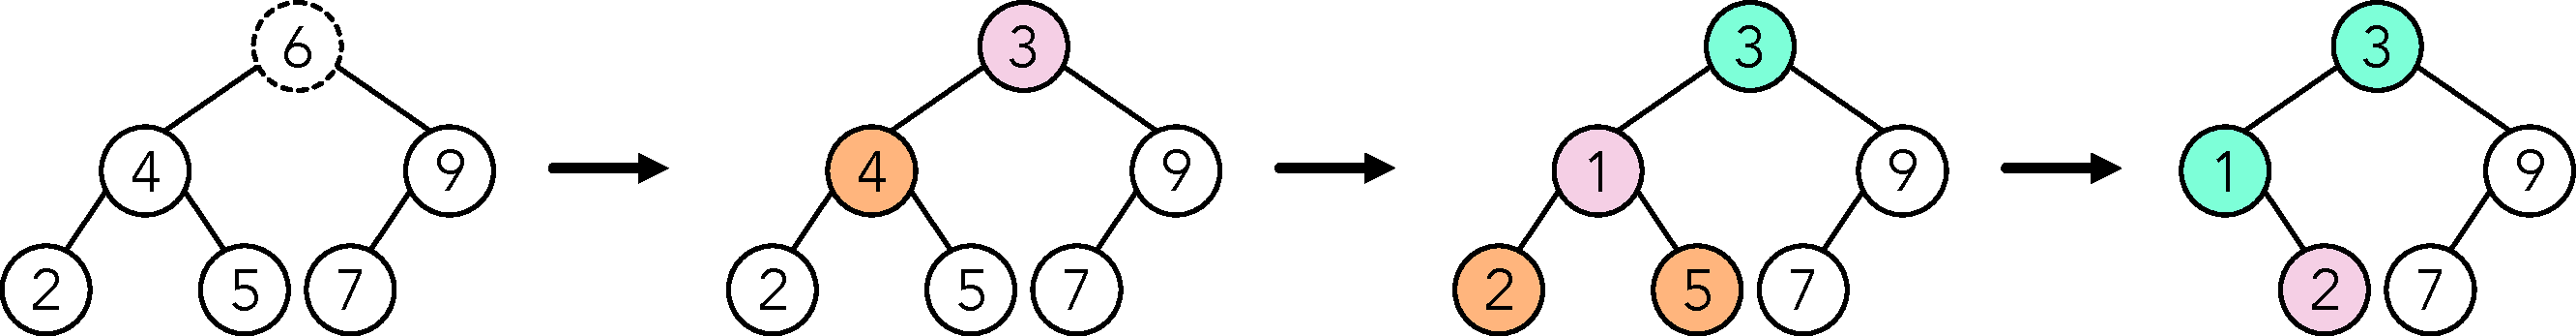
\includegraphics[width=.6\textwidth]{assets/mutate-diagram.pdf}
  \caption{Validity-preserving mutation of a binary search tree, maintaining the
  BST invariant.}\label{fig:mutation}
\end{figure}

\noindent {\em Example-Based Tuning} Earlier we pointed out that good generators
produce ``realistic'' inputs; one way to ensure this is to tune the generator so
it produces values that are similar to some user-supplied values deemed
realistic. Existing tools make good use of this example-based approach to
tuning~\cite{soremekun2020inputs}, but they do not work with generators as
powerful as monadic generators. We implement a similar algorithm using
reflective generators: we can (1) again, reflect on the choices that lead to a
set of realistic values, and (2) run the generator with {\em new choice weights}
informed by the choices that we saw.

Both of these applications have the potential to significantly improve testing
effectiveness, and we get {\em both} by upgrading our existing generators to
reflective ones. Additionally, we are confident that there are more use-cases
for reflective generators, which we discuss more in the following sections.

\subsubsection{Proposed Work: Bringing Fuzzing into Focus}
{\em Fuzzers} like AFL~\cite{afl-readme} use principles that are similar to the
ones behind PBT: they both leverage randomized testing to quickly exercise
as many program behaviors as possible.

One might then expect that the fuzzing and PBT share a significant amount of
literature, but in reality they do not. Often the communities seem to ``talk
past'' one another.

We propose that the main thing separating the PBT and fuzzing communities is
simply a difference of {\em focus}. The fuzzing literature mostly talks about
fast and automatic ways to find critical (security) vulnerabilities in
programs---usually manifesting in the form of crash failures.  In contrast, PBT
researchers want effective ways to test semi-formal logical specifications of
their programs. Both areas of focus are important: fuzzing captures the ``80\%''
of cases catching high-profile bugs with minimal programmer effort, and PBT
gives a level of thoroughness that fuzzing does not claim to match. But there is
something unsatisfying when things are laid out this way. In particular, while
fuzzing and PBT focus on different testing problems, they face many of the same
technological hurdles. Both PBT and fuzzing need fast and effective ways to
generate random inputs that are valid for the systems that they are testing, and
neither community has truly settled on the ``right'' way to get there.

There is already some work at the intersection of PBT and fuzzing...
\cite{10.1145/3293882.3339002,
DBLP:journals/pacmpl/Lampropoulos0P19,DBLP:conf/icse/ReddyLPS20} \todo{Talk more
about hypofuzz and crowbar}

\begin{wrapfigure}{l}{0.5\textwidth}
  \centering
  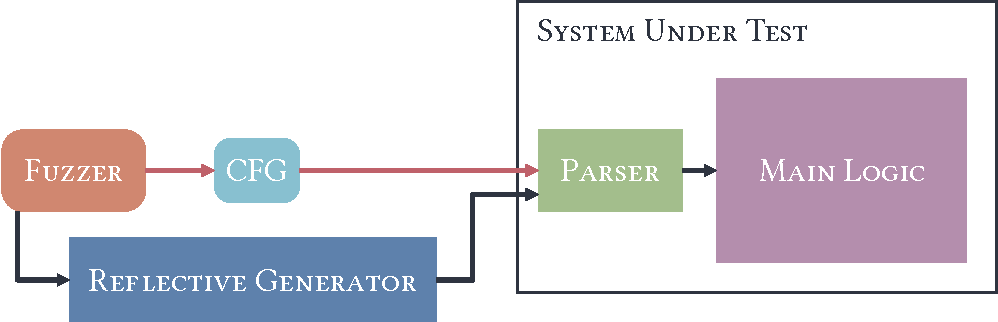
\includegraphics[width=.4\textwidth]{assets/fuzzing.pdf}
  \caption{Overview of gradually constrained fuzzing.}\label{fig:fuzzing-plan}
\end{wrapfigure}

Our system will start with a setup similar to Crowbar, but with a much greater
focus on the generators; in particular, we will use reflective generators to
gain significant testing power. The setup is shown in
Figure~\ref{fig:fuzzing-plan}. We start with a classic fuzzing setup, attempting
to make the system under test crash by passing it a variety of semi-random
inputs. Normally, the fuzzer is working against the parser, in the sense that
the parser's job is to reject invalid inputs and the fuzzer's job is to ``get
past the parser.'' The CFGs used by grammar-based fuzzers help a bit, but they
cannot generate inputs satisfying complex context-sensitive constraints. As in
Crowbar, we avoid this adversarial relationship and subsume grammar-based
generation with a powerful generator that is powerful enough to satisfy the
parser by construction; in our case, that generator is reflective.


Why use a reflective generator?  One compelling reason is that the backward
interpretation of the reflective generator can be used to help seed the fuzzer.
Most fuzzers ask for a number of {\em seeds}, input examples that the fuzzer can
start from, in order to ensure that the fuzzer does not spend ages exploring
inputs that have no hope of working out. Normally these seeds are easy enough
for the user to write down, since they are simply program inputs, but now that
we are asking the fuzzer to generate sequences of choices it becomes much more
tedious (and error prone) to produce seeds by hand.  This is one great use for a
backward interpretation. The user can write down their seeds (either as values
in the program, or as text that can be parsed by the program's parser), and then
the reflective generator can reflect on the choices that produce those seeds.

The reflective generator also provides validity-preserving mutation  Guided by
heuristics, the system can opt to supplement the fuzzer's mutation schedule with
mutations that are obtained by the reflective generator's validity-preserving
mutation. \todo{Say more}

\todo{Talk about the grand vision of gradually constrained fuzzing, and make
sure to talk about implementation language}
% The flagship feature of this approach is that a reflective generator is far more
% powerful and flexible than a CFG when it comes to constraining the generated
% inputs. At its simplest, a reflective generator can enforce the same invariants
% as a simple CFG, ensuring that the input is well-formed (and, since the
% reflective generator lives in the same language as the system under test,
% well-typed). But we need not stop there. If the tester finds that the fuzzer
% still fails to produce useful inputs, the user is free to add constraints to the
% reflective generator.  These constraints can be simple, like narrowing the range
% of an integer field, or extremely complex, like ensuring that a program is
% well-typed. The beauty is that the tester can decide exactly how hard to work on
% the generator, finding the the right balance between effort and testing
% performance.

% Of course, if a tester was only concerned with satisfying input constraints,
% they might just opt to write a standard PBT generator. Another benefit of this
% approach is that it keeps an off-the-shelf fuzzer in the loop, using its
% highly-tuned process for coverage-guided mutation to help make choices
% intelligently. In theory, this may mean that the user can stop optimizing the
% generator early, allowing coverage information to guide the generator the rest
% of the way.

% One interesting note is that there is flexibility in exactly how we tell the
% generator to process choices. We could choose to interpret the reflective
% generator as a strict parser (albeit of a much simpler language) and reject
% invalid choice sequences. Alternatively, we could interpret the reflective
% generator in a way that more robust to invalid choice sequences. It's possible that
% each could be better in different circumstances, so I am eager to experiment
% to see which makes the most sense.

\todo{Expand this a bunch}
Bringing PBT ideas to fuzzing, as I propose in Part 1, has the advantage that
advancements to PBT can directly improve fuzzing. It would be great if the
reverse was true as well! The FuzzChick library in Coq has already shown that
using fuzzing techniques to test properties is
worthwhile~\cite{DBLP:journals/pacmpl/Lampropoulos0P19}, so what would it look
like to bring properties into the system that I outlined in Part 1?

The answer is actually very simple: fuzz a binary that checks the property and
crashes if it fails. This can be done relatively easy with macros or build
scripts, so the programmer hardly needs to know that there is fuzzing happening
at all.  Ultimately this part of the project is not groundbreaking, but I think
the contribution lies in the unification of the ecosystems.

\subsubsection{Proposed Work: Reflective Shrinking}
A more modest application of reflective generators uses them to implement
validity-preserving {\em shrinking} of values to find smaller counterexamples
and speed up debugging. On its face, this feels similar to validity-preserving
mutation: Can we reflect on choices, shrink the choices, and then re-run the
generator with the smaller choices? Likely yes! But there are complications.
When mutating, it is often fine if the mutated value is accidentally quite
different from the original value, since the mutator is trying many values and
any that catch a bug are equally good. But when shrinking, it is often very
important to get another input that is both smaller and, ideally, provokes the
{\em same bug}. These nice properties are likely within reach, but care will
need to be taken to ensure that shrinkers behave as expected.

\subsection{Validation: Step 3, Understanding Testing Effectiveness \pagebudget{3}}
\subsubsection{Ongoing Work: Empirically Evaluating PBT Tools}

\subsubsection{Proposed Work: Visualizing and Tuning Data Distributions}

Plan of work: easily computable summary statistics; as well as user-defined
metrics for understanding what you care the most about from the distribution.
Seeing what the “average” data structure is that is getting generated. For
multimodal data, what are the different modes of data. The set of data types to
be handled in PBT are: algebraic data types, lists, trees (this would also cover
programs). Joe thinks we already have good visualizations for numbers, booleans,
and strings; it is compositional data types that we lack good visualizations
for. People need to (1) see representative examples (2) understand spread (3)
indicate areas of the space that should not be explored.  \bcp{I love this
thread---understanding the distribution that you're getting from a random
generator is one of the most challenging aspects of PBT---the thing that makes
it an art rather than a pushbutton or even fully automatable activity.  (We
should acknowledge this challenge even more clearly and prominently, at the very
top.)  Jessica and I have been struggling just this week to figure out what to
measure to get a better understanding of some specific distributions!  I feel
like there must be a ton or two of work on this, in adjacent or distant
communities.  I wonder how we'd find it...} \amh{Currently the project ideas are
arranged chronologically according to when programmers would use them (i.e.,
first they would write properties, then generators, then understand their
solutions, then integrate the tests into continuous integration, etc.). I could
see also ordering by our level of enthusiasm / likelihood to work on it, which,
as I understand, would put this section at the top.}

Plan of work: indicating areas of the distribution that should not be generated.

Example: writing a generator of programs (for instance, to test out a compiler).
You want lots of different programs that make sense in different ways. You want
large ones, small ones, ones that use variables in coherent ways, ones that
don’t overuse certain constructs, ones that use a variety of different language
features. You want the generated programs to be representative of those that
people might write. You also want some weird programs to catch the edge cases,
but you don’t want all weird programs. (How big, how deep, how wide of
programs?). Also, for trees, one might want to specify heights and breadths of
the tree.


\subsubsection{Proposed Work: Debugging Support for Understanding Counterexamples}

Once a PBT tool generates a counterexample of where a property fails, a
programmer will need to understand what in an input caused the program to fail.
This task can be rather challenging because generated inputs can be complex,
deep data structures \todo{Do we have a reference that implies the complexity of
generated counterexamples?}. Methods for making it clearer why a counterexample
fails could be to generate additional inputs that are very close to the
counterexample that are actually correct, to run the program up to the point
where the traces of the programs begin to diverge, and then to drop a programmer
into a debugging environment where they can query the state of the program and
step through the remainder of the execution. PI Head has prior work designing
debugging tools that help programmers understand trace divergences in an
educational setting~\cite{suzuki2017tracediff}.  \bcp{This sounds very cool!  We
should acknowledge all the work that's been done on shrinking in the PBT
community.} \amh{Good thinking!}
\hg{Hila had a similar idea that she wanted one of her undergrads to work on, we
should make sure we don't step on toes}

\subsubsection{Proposed Work: Integration with Continuous Integration Workflows}

The preliminary study suggests that one area that new developer tooling may be
needed is in managing the interplay between PBT and continuous integration (CI)
systems. Recall that developers we spoke with pointed out frustration with the
fact that PBT is both nondeterministic and long-running. This combination left
them unsure of exactly where and when to test their properties: testing
properties locally slowed down their workflow, but testing them in CI
occasionally led them to find bugs at inconvenient times.

It is likely that PBT tools could play a role in improving this state of
affairs. For example, one could take inspiration from some theorem
provers~\cite{berghofer2004random} and create a system in which properties are
checked locally but in the background, as the programmer works on other things.
This avoids waiting time while potentially being less frustrating than running
in CI, since bugs would likely be found while the programmer still had the code
``paged in.'' Alternatively, one might design a PBT system with CI in mind,
providing automated features for deferring property failure notifications until
a specified time or turning failing properties into unit tests that can be saved
for future testing.

If the full-scale study indicates that this would be a useful line of work, we
will refine these ideas via user-centered design. Rather than build a system and
hope users like it, we will build minimal prototypes and iterate on the design
by observing testers using it. Ultimately we hope this will guide us to a tool
that will meaningfully improve the experience of PBT.

\subsection{Education: Advancing Testing in the Broader Culture \pagebudget{1}}

The preliminary study also reminded us that PBT builds on concepts that are not
always comfortable for developers, and we expect that we will learn more about
the specifics of that discomfort in the large-scale study.  Prior work has
explored ways to close this knowledge
gap~\cite{wrenn2021using,nelson2021automated}, but we expect there are further
education challenges that are worth exploring.

I hope to work with the course staff of CIS 1210 to incorporate PBT into the
curriculum. The ideal scenario would be to add a PBT thread throughout the
course, giving students the tools to specify and test their code as they go.  I
plan to follow the lead of others who have done similar things before (e.g., the
PL folks at Brown University) to give students the best chance at incorporating
PBT into their tool-set.

There are a few important challenges that need to be considered in order for
this to work out.  The curriculum is already quite full, so adding PBT likely
means removing something else. I will need to work with the professors currently
teaching the course to find room, but I expect that this process will be fairly
difficult. It is also possible that adding PBT will actually make parts of the
course {\em easier}, especially for students with some knowledge of logic and/or
less well-developed unit testing instincts. Honestly I think this is a good
thing, as it gives students more ways to succeed and it may re-enforce the value
of PBT, but some may find this problematic.

\subsection{Plan of Work \pagebudget{1}}

\todo{(with a pretty pert chart or suchlike...)}

\subsection{Broader Impacts \pagebudget{.5}}
The Project Description must contain, as a separate section within the narrative, a section labeled ``Broader
Impacts of the Proposed Work". This section should provide a discussion of the broader impacts of the proposed
activities. Broader impacts may be accomplished through the research itself, through the activities that are
directly related to specific research projects, or through activities that are supported by, but are complementary to
the project. NSF values the advancement of scientific knowledge and activities that contribute to the
achievement of societally relevant outcomes. Such outcomes include, but are not limited to: full
participation of women, persons with disabilities, and underrepresented minorities in science, technology, engineering, and
mathematics (STEM); improved STEM education and educator development at any level; increased public
scientific literacy and public engagement with science and technology; improved well-being of individuals in
society; development of a diverse,globally competitive STEM workforce; increased partnerships between
academia, industry, and others; improved national security; increased economic competitiveness of the United
States; and enhanced infrastructure for research and education.

\subsection{Results from Prior NSF Support \pagebudget{.5}}
If any PI or co-PI identified on the project has received NSF funding (including any current
funding) in the past five years, in formation on the award(s) is required,
irrespective of whether the support was directly related to the proposal or not.
In cases where the PI or co-PI has received more than one award (excluding amendments),
they need only report on the one award most closely related to the proposal. Funding includes not just salary
support, but any funding awarded by NSF. The following information must be provided:\\

\noindent
\emph{\underline{Name of PI}}: NSF-Program (Award Number) ``Title of the Project'' (\$AMOUNT, PERIOD OF SUPPORT).
{\bf Publications:} List of publications resulting from the NSF award. A complete bibliographic citation for each
publication must be provided either in this section or in the References Cited section of the proposal); if
none, state: ``No publications were produced under this award.'' {\bf Research Products:} evidence of research products
and their availability, including, but not limited to: data, publications, samples, physical collections, software,
and models, as described in any Data Management Plan.

% \subsubsection{Proposed Study}
% The Project Description should provide a clear statement of the work to be undertaken and must include:
% objectives for the period of the proposed work and expected significance; relation to longer-term goals of the PI's
% project; and relation to the present state of knowledge in the field, to work in progress by the PI under other
% support and to work in progress elsewhere.
%
% The Project Description should outline the general plan of work, including the broad design of activities to be
% undertaken, and, where appropriate, provide a clear description of experimental methods and procedures.
% Proposers should address what they want to do, why they want to do it, how they plan to do it, how they will
% know if they succeed, and what benefits could accrue if the project is successful. The project activities may be
% based on previously established and/or innovative methods and approaches, but in either case must be well
% justified. These issues apply to both the technical aspects of the proposal and the way in which the project may
% make broader contributions.

\subsectionstar{More stuff to not forget :-)}

Unfunded collaborations: Any substantial collaboration with individuals not included in the budget should be described in the Facilities, Equipment and Other Resources section of the proposal (see Chapter II.C.2.i) and documented in a letter of collaboration from each collaborator. Such letters should be provided in the supplementary documentation section of FastLane or Research.gov and follow the format instructions specified in Chapter II.C.2.j. Collaborative activities that are identified in the budget should follow the instructions in Chapter II.D.3.

Remember to not use any URLs in the project description!  (They are
encouraged in the references.)
